\documentclass[dvipdfmx]{jsarticle}
%\documentclass[a4j]{ujarticle}
\usepackage{resume}  % resume用スタイル
\usepackage{udline}  % 下線用
\usepackage{comment} % 複数行コメント

\pagestyle{plain}

\begin{document}
\twocolumn[
    \beginheader{令和5年度 コンピュータサイエンス研究II 中間審査会}{2023}{8}{8}{井上研究室}
    \title{TravelatAR : 地表面近似テクスチャーのアニメーション重畳表示よる\\歩行速度制御システム}
    \affiliation{東京工科大学大学院 バイオ・情報メディア研究科 コンピュータサイエンス専攻}
    \author{G2122014 島谷~~優佑}
    \endheader
]

\vspace{3mm}
%\setcounter{page}{1}

%------------------------------------------------------------------
\section{はじめに}
イベント会場やターミナル駅のホームは多くの人で溢れかえっている.
歩行者一人ひとりの歩行速度をコントロールすることは、そうした混雑した公共空間での歩行者同士の事故を減らすことにつながる.
多くの場合、現場に配置された警備員が音声警告や看板で群衆に注意を促している.
しかし,人によっては無視して従わない場合や,見落としてしまう場合がある.
また,従う人に対しても,指示の意味を解釈して行動に移す必要があり,心的コストが要求される.
このような場面では,直感的にわかる注意,誘導方法が望ましい.


人は五感によって得られる情報のうち,87\%を視覚から得ている\cite{book1}.
そのため視覚は行動に大きな影響を及ぼすことが知られている.
視覚により人の行動に影響を与える例として,曲線の描かれたカーペットを床に敷くことで床が歪んでいるように見せ走りづらくさせる工夫が存在する\cite{webpage1}.
このように,床のテクスチャを変化させることで人の行動に影響を与えることが可能であるため,直感的にユーザが理解できる注意,誘導が可能でないかと考えられる.


通路や道路に床テクスチャを提示する際,実際に床の上にテクスチャを設置することは設置や撤収が大変である.
また,大勢の人が様々な方向に向かって歩く商店街などの大通りではプロジェクターによる正しい歩行誘導をできる形の床テクスチャ提示は困難である.
そこでARを用いることで,個人個人に道を問わず歩行誘導をできる形の床テクスチャ提示ができる.


ARを用いた歩行者誘導についての研究で塚本らの拡張現実感を用いたテクスチャ変更による人物行動制御手法が存在する.
この研究ではARグラスを用いてユーザの視界に存在する床に動くムービングウォークのテクスチャを提示することで行動制御を試みた.
結果として影響が大きく得られなかった要因として実世界の床が見えてしまったことが原因の一つと考えられている\cite{article1}.


本研究ではARを用いた行動制御方法では床に現実にを模していないバーチャル床をアニメーション重畳表示して見せるより,現実の床を模したバーチャル床をアニメーション重畳表示した方が没入感が高まり,ユーザの動きをより制御できると考える.
本稿では芝生道にて,芝生を模したバーチャル床を表示した場合,芝生を模していないバーチャル床を表示した場合を比べてユーザの歩行速度制御に優位性が出るか否かの調査を行う.

%------------------------------------------------------------------
\section{travelatAR}
本研究ではユーザの視界に映る床に現実の床を模したバーチャル床をアニメーション重畳表示するシステムを提案する.


\subsection{システム概要}
図\ref{fig:gaiyo}に本システムの概要を示す.
本システムでは被験者にARグラスを装着してもらう.
これにより,現実の床を模したバーチャル床ををユーザの視界にアニメーション表示する.
\begin{figure}[t]
    \centering
    \fbox{
    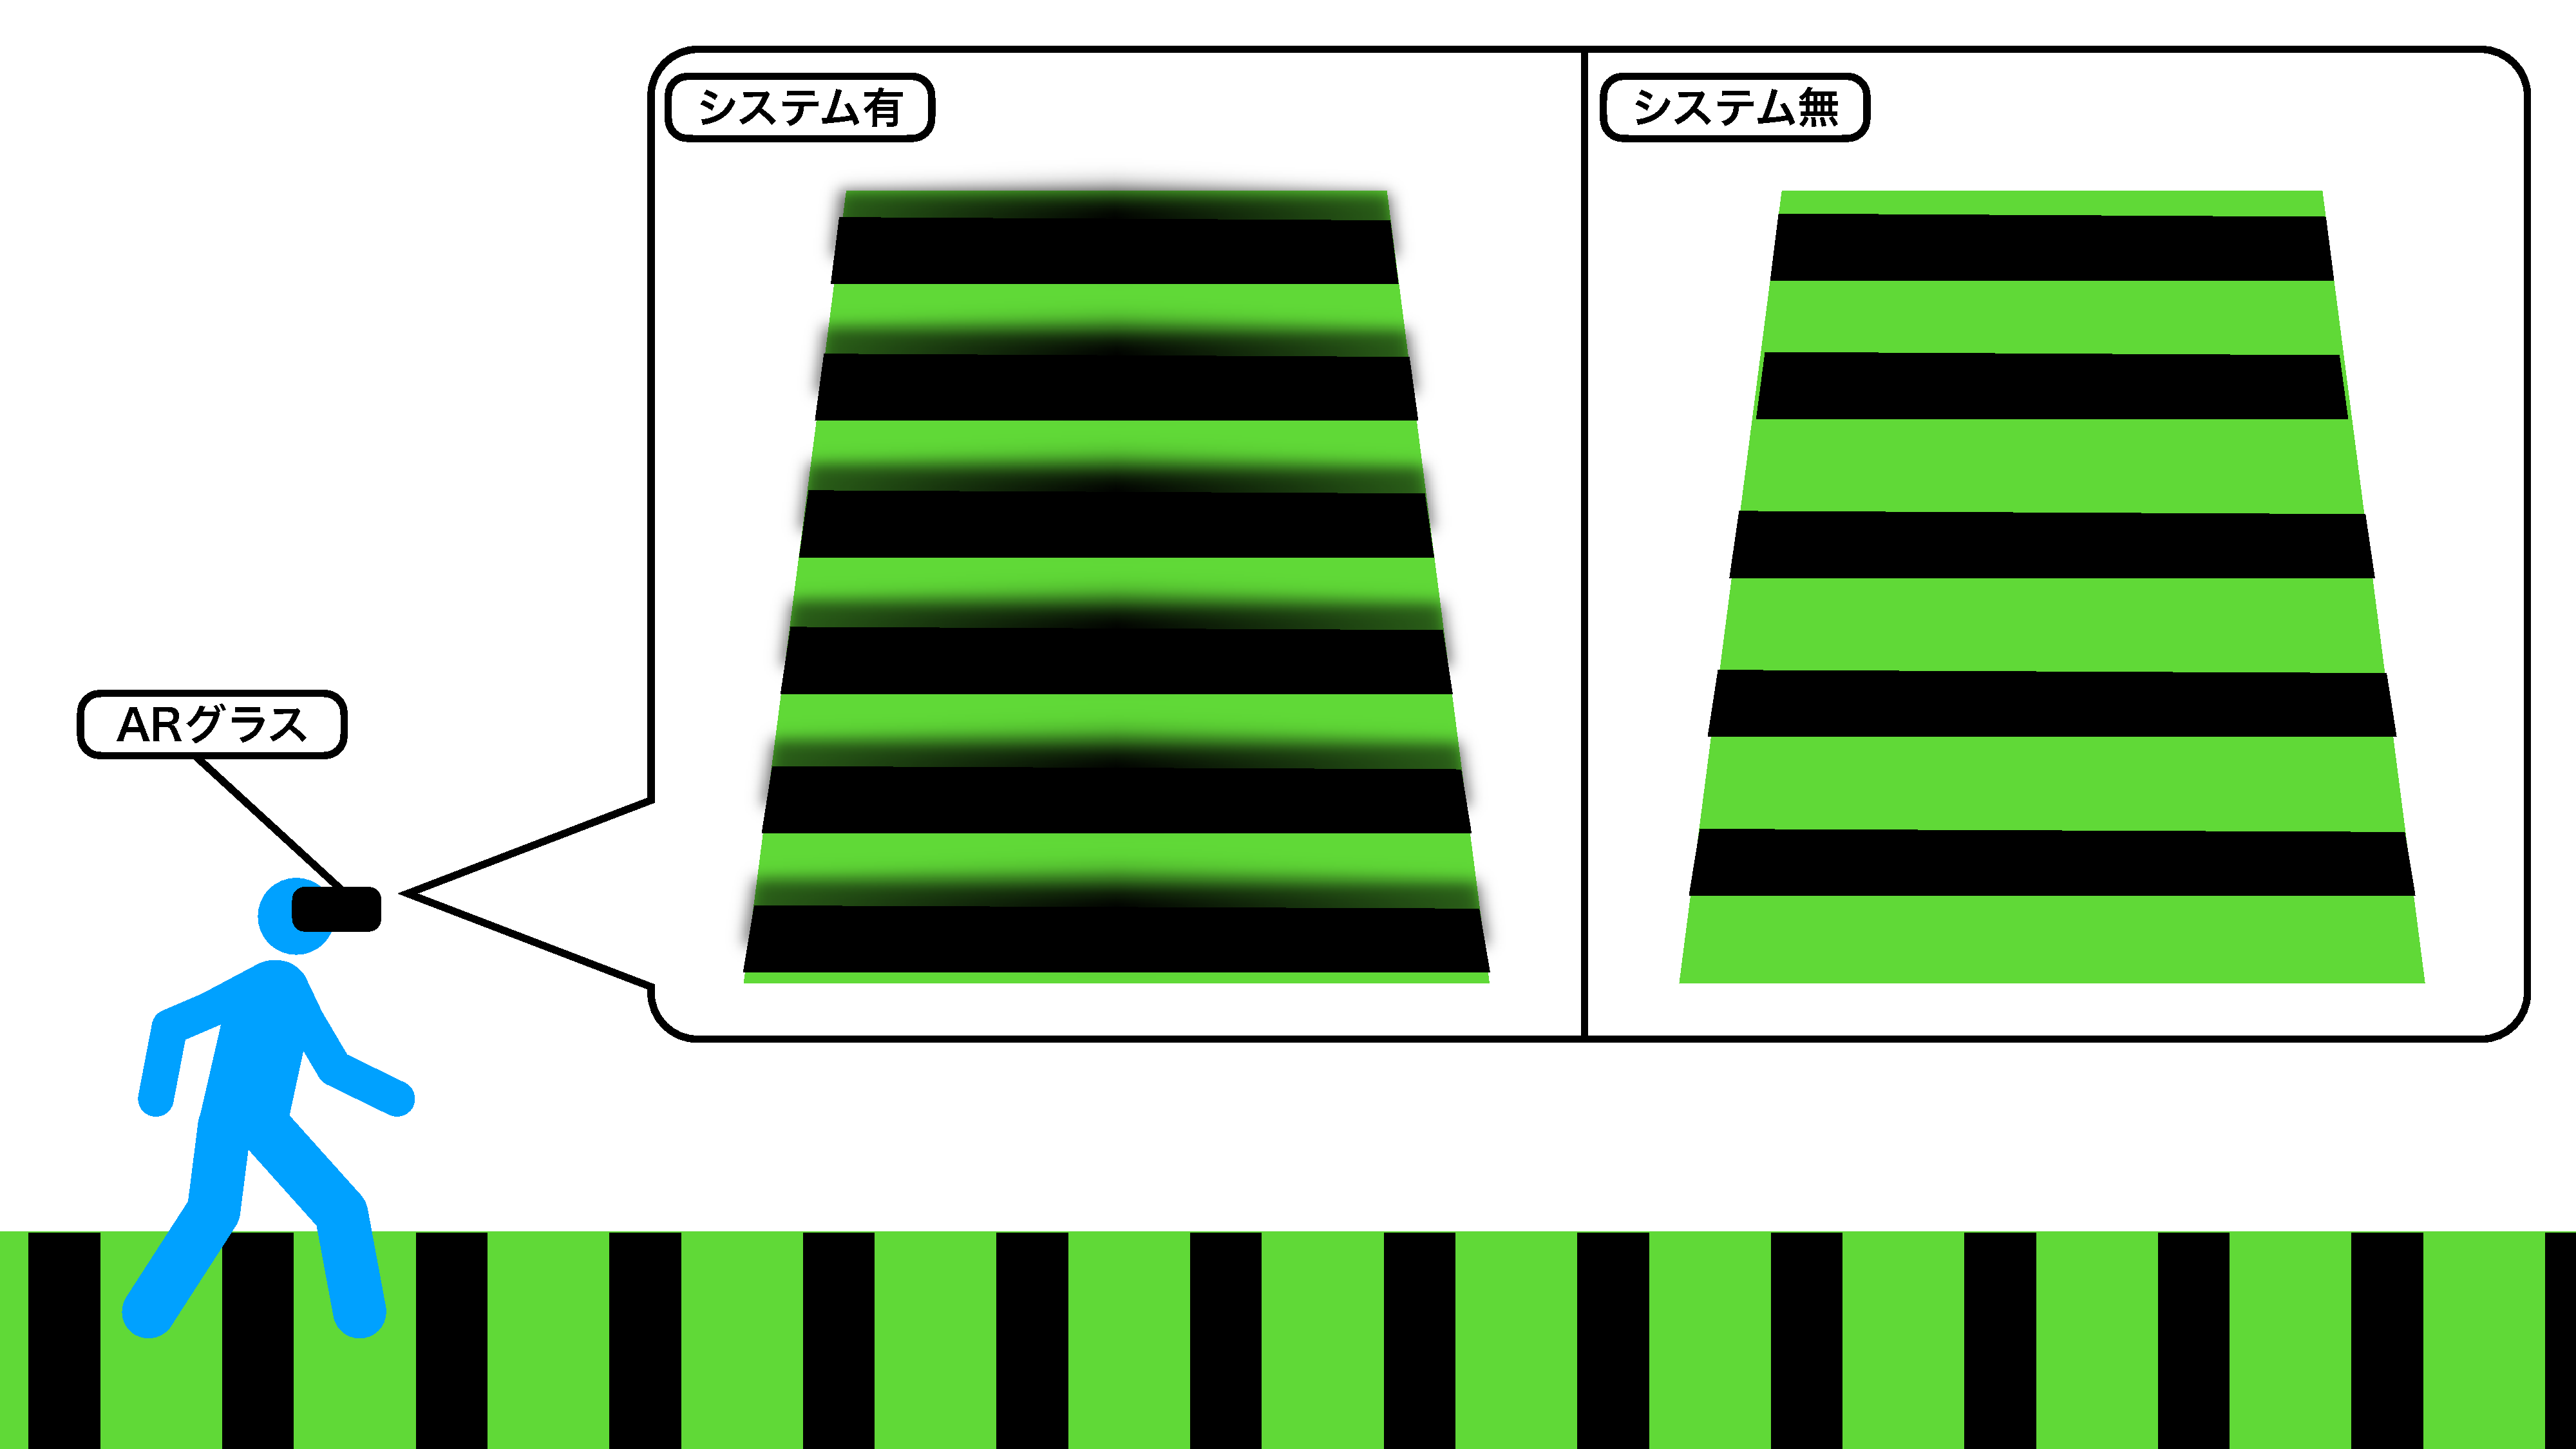
\includegraphics[width=1.1\linewidth]{fig/gaiyo.pdf}
    }
    \caption{システム概要図}
    \label{fig:gaiyo}
\end{figure}

\subsection{リアルテクスチャ}
\begin{figure}[htbp]
    \centering
    \fbox{
    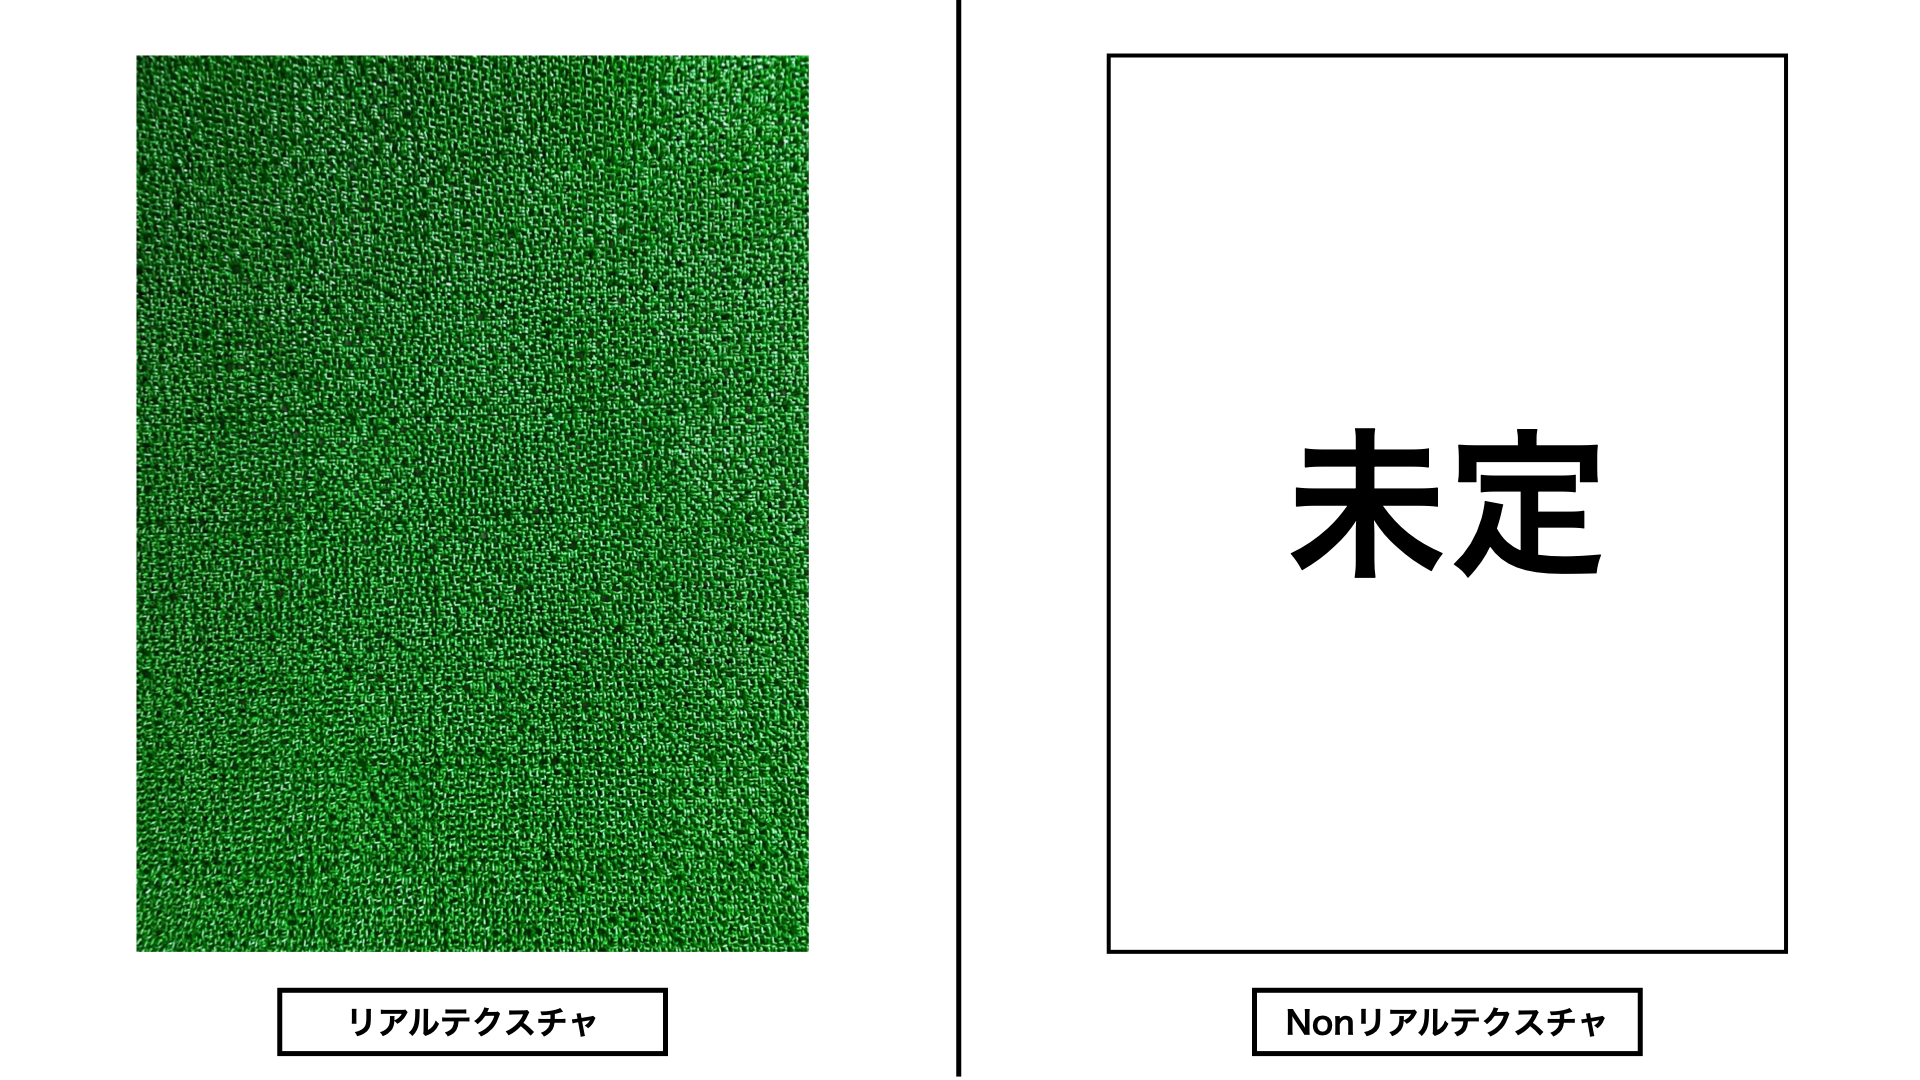
\includegraphics[width=1\linewidth]{fig/texture.jpeg}
    }
    \caption{バーチャル床のテクスチャ}
    \label{fig:texture}
\end{figure}
図\ref{fig:texture}の左にに今回作成したリアルテクスチャを示す.
また、評価実験の際にリアルテクスチャの比較対象としてNonリアルテクスチャを使う予定だが未定である.
今回提示したリアルテクスチャは人工芝の道を歩くことを想定し作成した.
本システムでは,これらのテクスチャをバーチャル床にアタッチし被験者の視界の床にアニメーション重畳表示を行う.

\subsection{プロトタイプ}
\begin{figure}[t]
    \centering
    \fbox{
    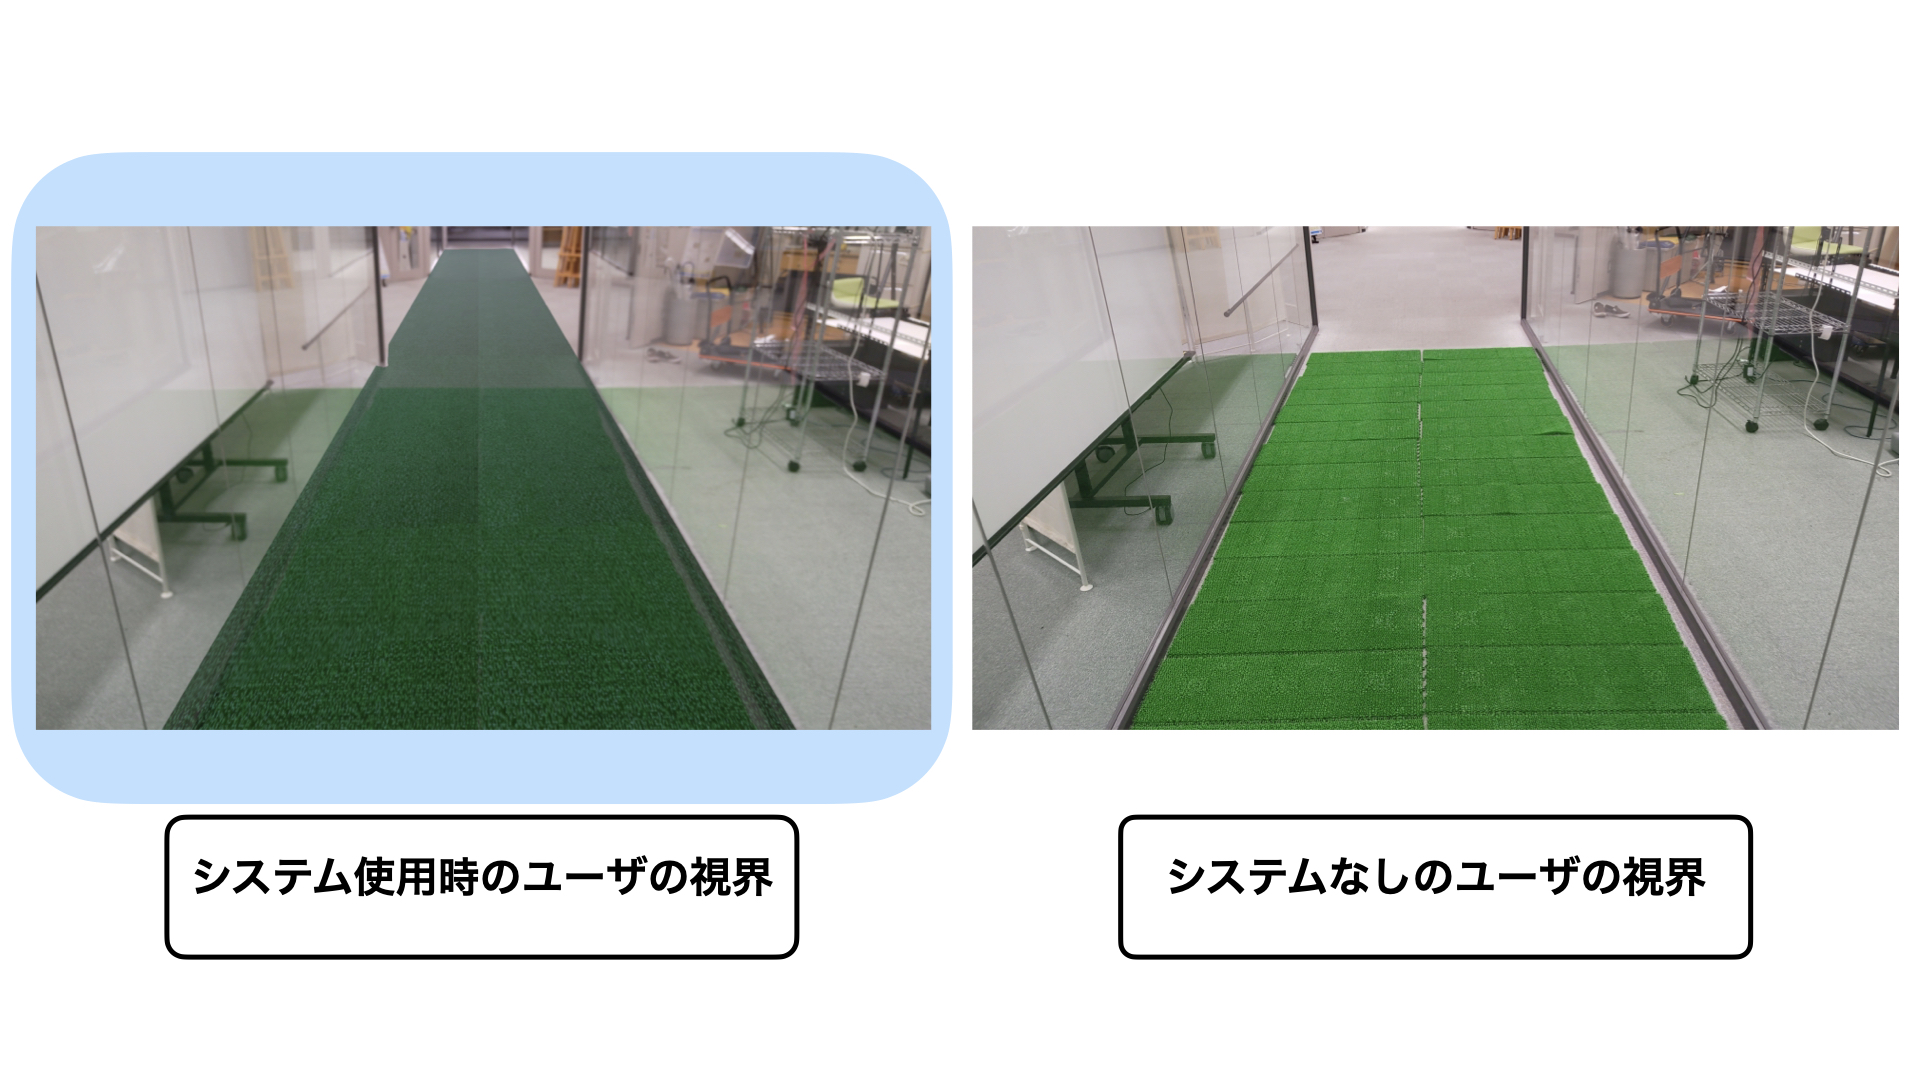
\includegraphics[width=1\linewidth]{fig/proto.jpeg}
    }
    \caption{プロトタイプ}
    \label{fig:puroto}
\end{figure}
図\ref{fig:puroto}に本システムのプロトタイプを示す.
プロトタイプでは上記の芝のリアルテクスチャをバーチャル床にアタッチし,床にアニメーション重畳表示を行なった.
バーチャル床はユーザの約20m前からこちらに向かうように動いてくる.
%------------------------------------------------------------------
\section{実験方法}

本稿では芝生道にて,芝生を模したバーチャル床を表示した場合,芝生を模していないバーチャル床を表示した場合を比べてユーザの歩行速度制御に優位性が出るか否かの調査を行う.
実験環境を図\ref{fig:kokaton}に示す.被験者は頭にはARグラスのHololens2を,体にはスマートフォンを揺れないように固定して装着してもらう.
実験手順を以下に示す.
\begin{enumerate}
    \item システムを使用していない状態のHololens2をつけてもらい,指定した道を指定距離歩いてもらう.
    \item 本システム(リアルテクスチャ or 模様なし)を使用して歩いてもらう
    \item 手順2とは違うバージョンを使用して歩いてもらう
\end{enumerate}

\begin{figure}[t]
    \centering
    \fbox{
    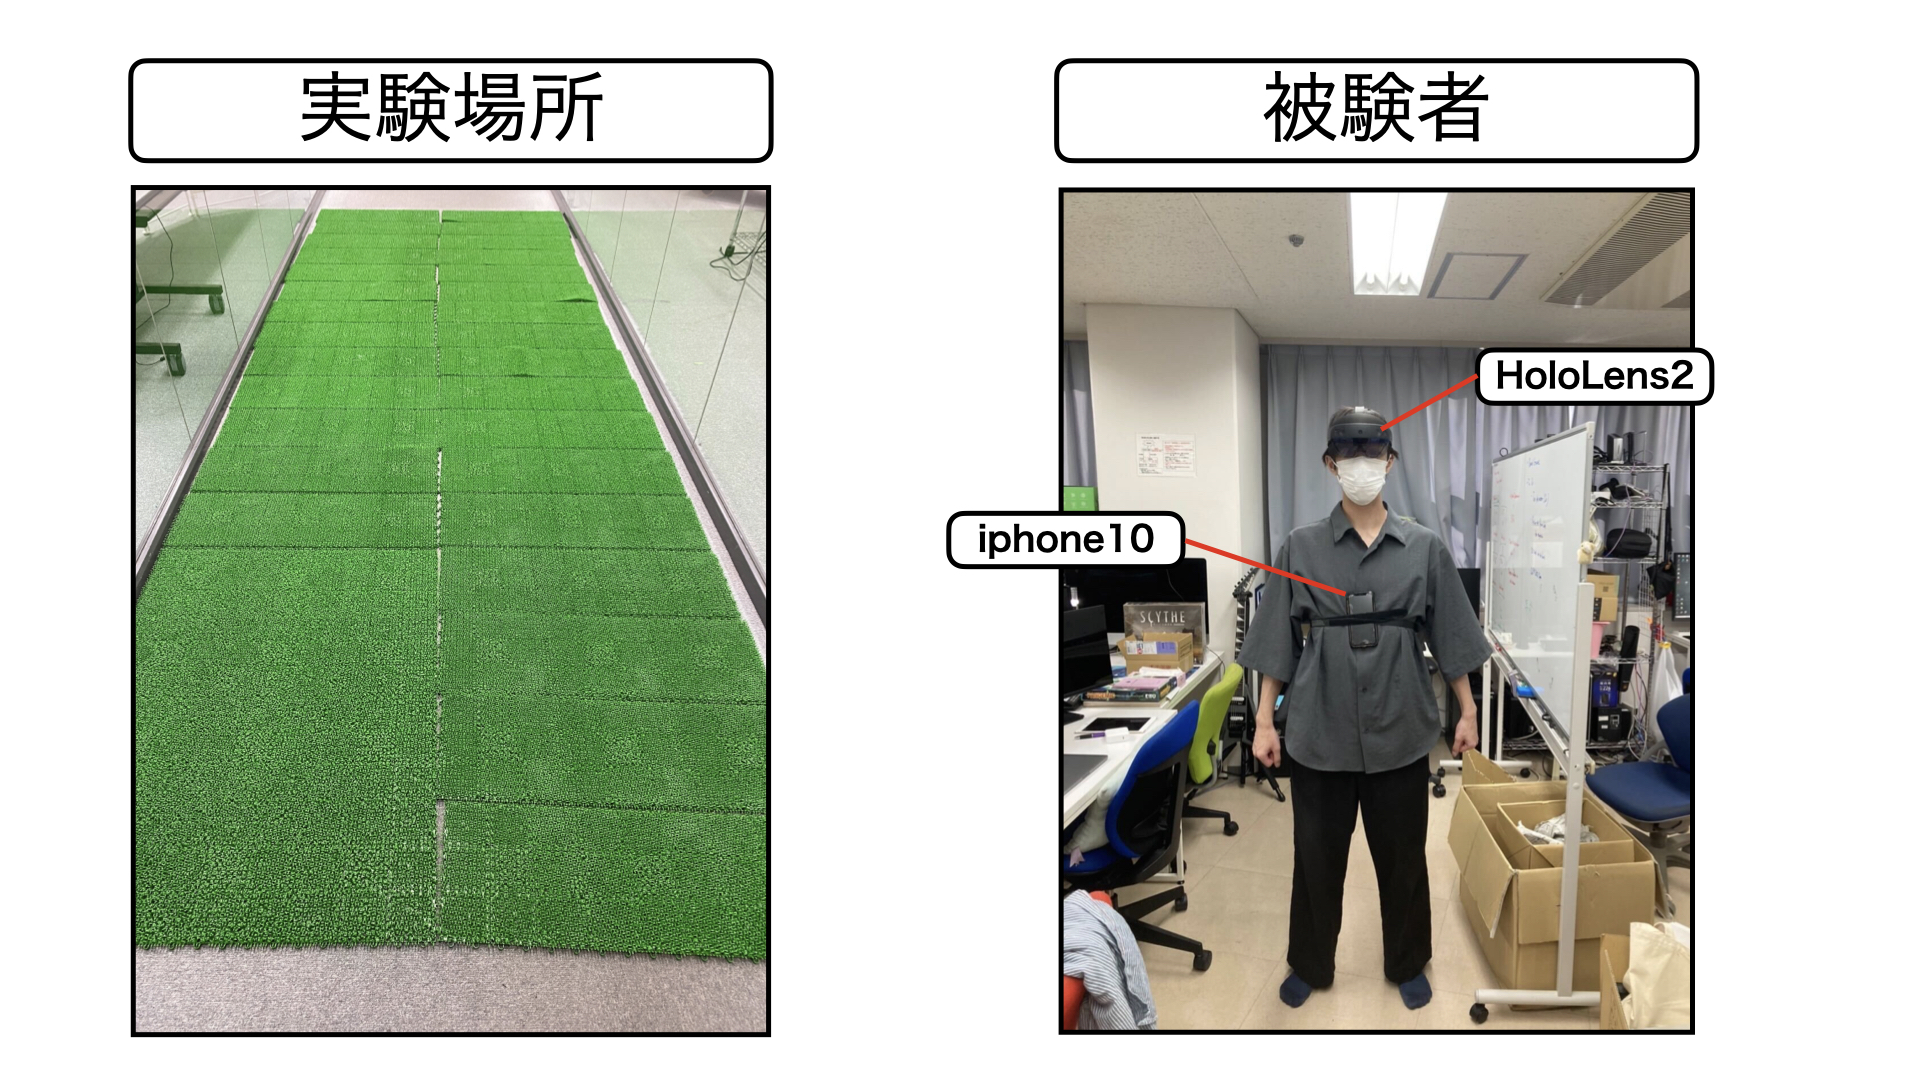
\includegraphics[width=1\linewidth]{fig/enviroment.jpeg}
    }
    \caption{実験環境}
    \label{fig:kokaton}
\end{figure}

 \subsection{評価方法}
 感性評価では、歩行後に歩いている速度が速く感じるか,遅く感じるかといった感覚を速度感とし
 本システムを用いることで速度感に変化を感じたか.
 リアルテクスチャは本当に床が動いているように感じたかを
 5段階のリッカート尺度で回答してもらう.


 定量評価では,被験者の体に装着されたスマートフォンの加速度センサーを用いて,
 本システムを使用した時とシステムを使用していない時で被験者の歩行速度は変化するのかを評価する.

 %------------------------------------------------------------------
\section{まとめ}
本研究では,地表面近似テクスチャーのアニメーション重畳表示よる歩行速度制御システムを提案した.
今後の課題として,Nonリアルテクスチャの選定,本システムを用いた実験が挙げられる.
また,実験結果からバーチャル床のテクスチャや挙動の改善を行う.
%------------------------------------------------------------------
\bibliographystyle{junsrt}
\bibliography{ref}
\end{document}
